\documentclass[twocolumn]{article}
\usepackage{cite}
\usepackage{amsmath,amssymb,amsfonts}
\usepackage{algorithmic}
\usepackage{graphicx}
\usepackage{textcomp}
\usepackage[margin=0.5in,footskip=0.25in]{geometry}
\usepackage[toc,page,title,titletoc]{appendix}

\title{Analysis and prediction of the Irish housing market}

\author{
    Seán Healy, Soren Dreano\\
    \texttt{\{healys47,soren.dreano2\}@mail.dcu.ie}
    \footnote{This work was completed as part of the CA-660 module.}
}

\def\BibTeX{{\rm B\kern-.05em{\sc i\kern-.025em b}\kern-.08em
    T\kern-.1667em\lower.7ex\hbox{E}\kern-.125emX}}

\begin{document}

\maketitle
\begin{abstract}
Analysis of the housing market in Ireland is presented, beginning with the
evolution of both rent and purchase prices, and the multiple factors
influencing fluctuations in the last 10 years. Possible explanations for
changes will be presented, alongside with projections for future rental and
property prices, if current trends continue.
\end{abstract}\\\\
{\bf Keywords:} accommodation, housing, population, rent

\section{Introduction\label{s:intro}}

In the later part of the Celtic Tiger, a term referring to the economy of Ireland from the mid 1990s to the late 2000s, the Irish Property Bubble started to appear, which manifested itself as a constant and continuous rise in prices for almost a decade. In September 2008, the Irish government officially acknowledged the country's descent into recession\cite{kollewe08}, the collapse of the previously mentioned bubble being one of the major contributing factor to the global 2008 financial crisis. Unemployment rate rose from 6.5\% in July 2008 to 14.8\% 4 years later \cite{cso14} and house prices fell from 35\% between the end of 2007 and the end of 2010 \cite{environ10}.

Concerns around property prices began to rise a few years later, in mid-2012, as seen is figure 1, the number of queries on the Google search engine for the term "Property price" started surging in this period and costs continue escalating in Ireland \cite{kennedy21}.

\section{Methodology}
\subsection{Data sources}
Data from the Central Statistics Office and
WHEREVERYOUFOUNDYOURPDFIDONTRECALLTHEWEBSITE were used

\subsection{Software used}
To facilitate collaboration, we used a GitHub repository [6] to host the datasets and the code. As we were both familiar with Python3 and it has a large amount of libraries dedicated for data analysis and exploration, it is the language we went with. In term of libraries, we mainly used Pandas in order to parse and select the data sources, MatPlotLib to create graphical representation and Numpy.

\section{Results}
%\section{Evolution of the price in the housing market by county}
\subsection{Property price}
Unsurprisingly, the mean price to buy a property decreased from 2010 to 2012 after the Irish Property Bubble collapsed. The price surged drastically in most counties and most notably in Dublin, Kildare, Wicklow, Cork and Galway. This trend is shown clearly in figure 2. \begin{center}
\begin{tabular}{||c c||}
 \hline
 County & Increase in property price (\%) \\ [0.5ex]
 \hline\hline
 Dublin & 36.53 \\
 \hline
 Kildare & 36.49 \\
 \hline
 Wicklow & 34.43 \\
 \hline
 Cork & 20.37 \\
 \hline
 Galway & 11.44 \\ [1ex]
 \hline
\end{tabular}
\end{center}

\subsection{Rent price}
As shown in figure 3, the same pattern applies for the average renting price. Figure 4 presents a tight correlation between the evolution of both property price and rent cost.

\section{Factors}
\subsection{Population}
As shown in figure 5, population in Ireland is fairly stable. Indeed, from 2012 to 2016, population in Ireland increased slightly by 3.05\% while the mean property price increased by 15.83\%.

The increase in inhabitants might drive prices in the housing market up, as there will be more demand for the same number of accommodation. In order to test this theory, we looked at correlations between the total population of a county and the mean property price, from 2010 to 2016, for each county. Figure 6 is a kernel density estimation of the correlation and shows how much this correlation varies from county to county, with the mean being 0.309 and the standard deviation 0.369.

The Donegal, Leitrim, Roscommon, Sligo and Tipperary counties actually have a negative correlation between the evolution of property price and the evolution of the population. Figure 7 shows how these counties are outliers in the general trend.

The property prices decreased while the population continued to increase in all of the aforementioned counties.

\begin{center}
\begin{tabular}{||c c c c||}
 \hline
 County & Pop. 2016 & Pop. 2010 & Evolution \\ [0.5ex]
 \hline\hline
 Donegal & 159192 & 157748 & 1444 \\
 \hline
 Leitrim & 32044 & 30934 & 1110 \\
 \hline
 Roscommon & 64544 & 62248 & 2296 \\
 \hline
 Sligo & 65535 & 64378 & 1157 \\
 \hline
 Tipperary & 159553 & 155268 & 4285 \\ [1ex]
 \hline
\end{tabular}
\end{center}

\section{Conclusion}
The current Tánaiste Leo Varadkar recently said "One of our biggest deficiencies, in housing supply in Ireland, is we're a country of three-bed homes by-and-large and we don't have enough one-bed homes" \cite{mcgrath21}. We could not find any publicly available data on the matter. Nonetheless, an analysis on the housing supply in Ireland either by size or the number of bedrooms, especially in dense urban areas such as Dublin, Cork or Galway might confirm this deficiency. Further research should focus on the types of housing that sell the most and that have been constructed recently.

Appendixes, if needed, appear before the acknowledgment.

%[5]Central Statistics Office, <https://data.cso.ie/>
%[6]https://github.com/Gailenstorm/CA-660

\bibliographystyle{IEEEtran}
\raggedright
\bibliography{references}
\onecolumn
\appendices
\begin{figure}[h]
	\centering
    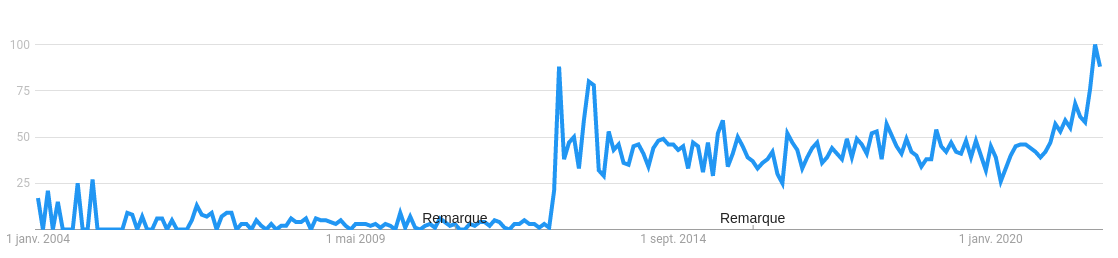
\includegraphics[width=0.47\textwidth]{../media/google_trend_property_price.png}
	\caption{Google Trends is a useful tool to see the evolution of the interest of a certain query on the Google search engine}
	\label{fig1}
\end{figure}

\begin{figure}[h]
	\centering
    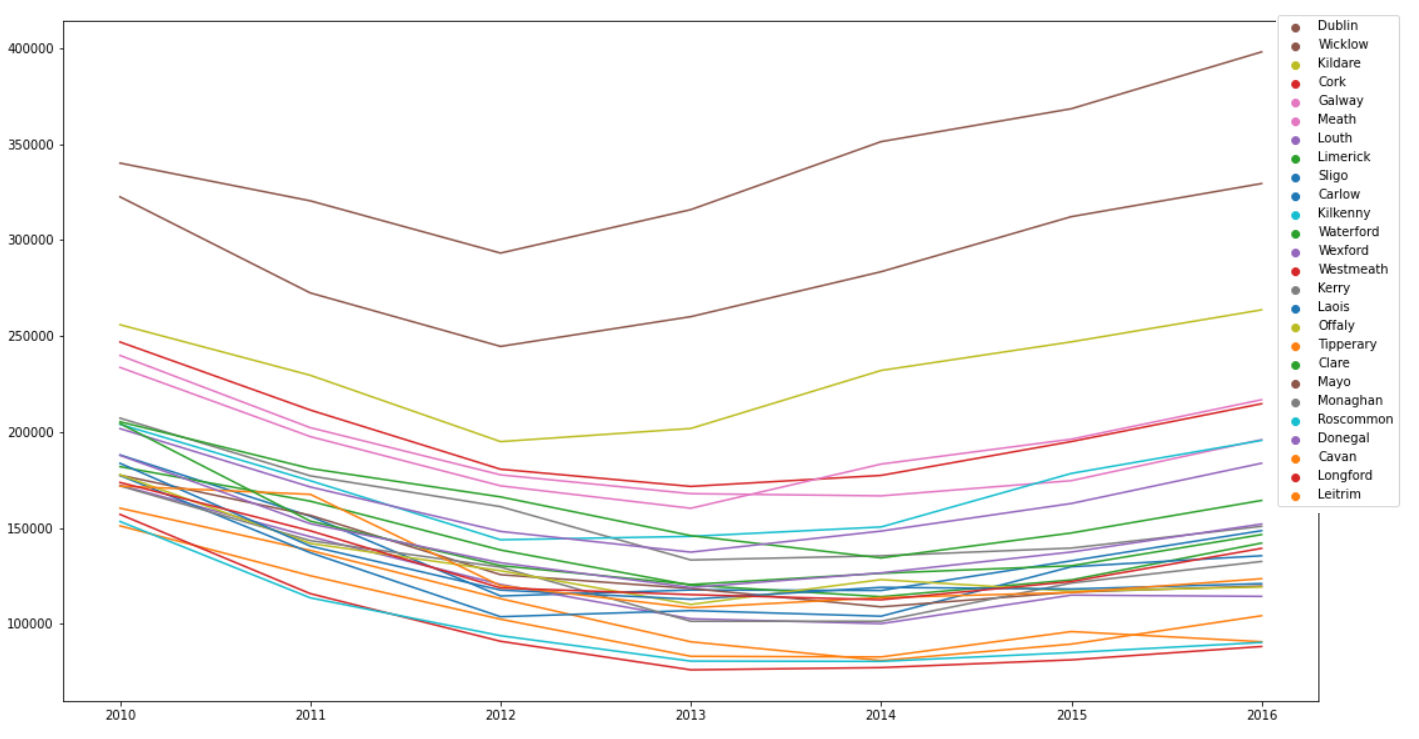
\includegraphics[scale=0.5]{../media/property_price.png}
	\caption{Average price for acquisition of property, by county, from 2010 to 2016}
	\label{fig2}
\end{figure}

\begin{figure}[h]
	\centering
    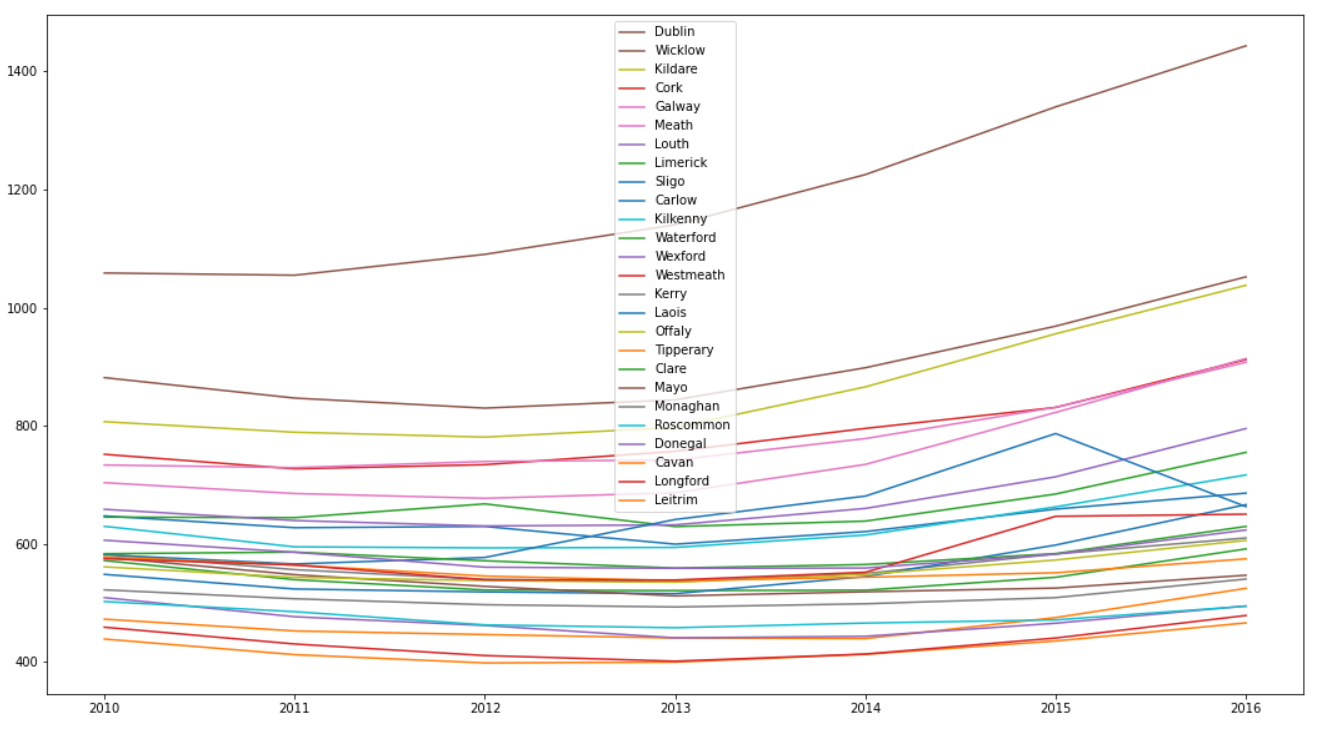
\includegraphics[scale=0.5]{../media/rent_price.png}
	\caption{Average price to rent a property, by county, from 2010 to 2016}
	\label{fig3}
\end{figure}

\begin{figure}[h]
	\centering
    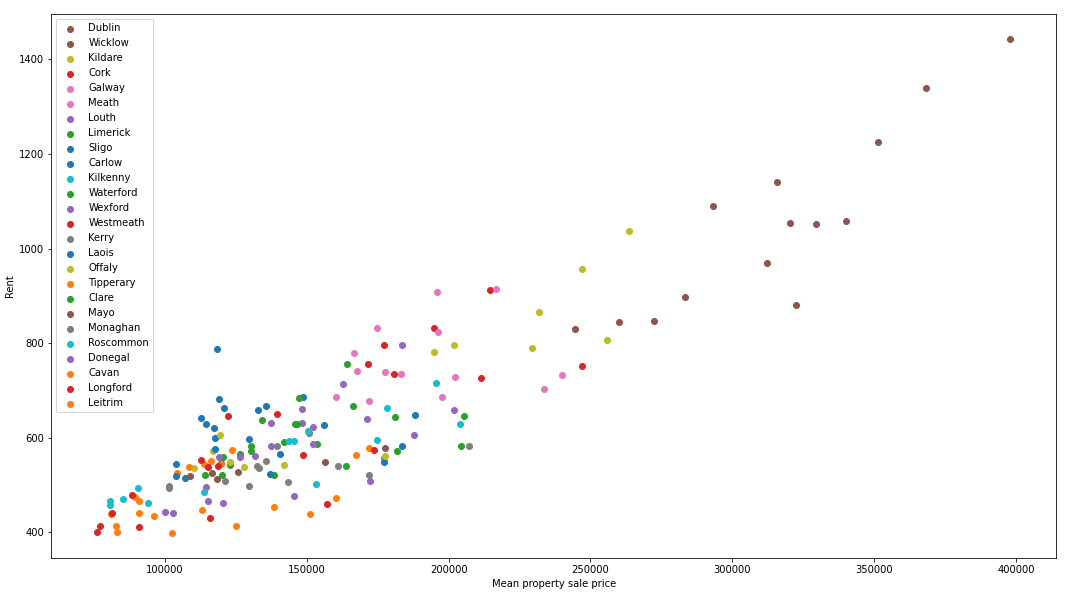
\includegraphics[scale=0.5]{../media/correlation_rent_acquisition.png}
	\caption{Rental price and property price are tightly linked}
	\label{fig4}
\end{figure}

\begin{figure}[h]
	\centering
    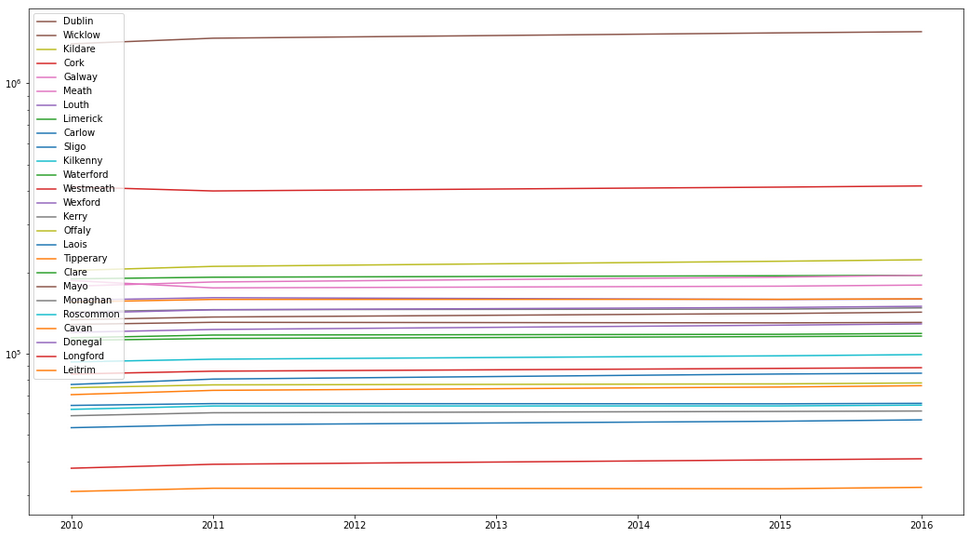
\includegraphics[scale=0.5]{../media/population_increase.png}
	\caption{Slight increase in population in Ireland from 2010 to 2016}
	\label{fig5}
\end{figure}

\begin{figure}[h]
	\centering
    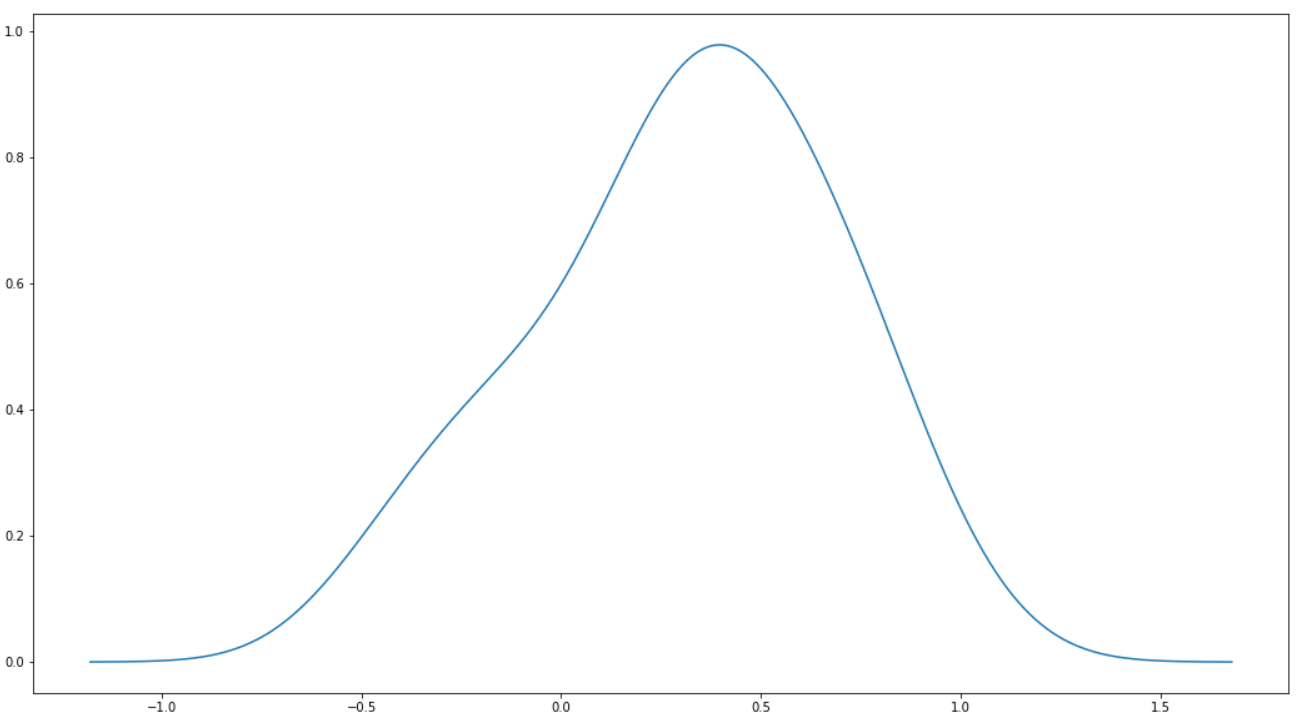
\includegraphics[scale=0.5]{../media/correlations_between_population_and_price.png}
	\caption{KDE of the correlations between population increase and price increase by county}
	\label{fig6}
\end{figure}

\begin{figure}[h]
	\centering
    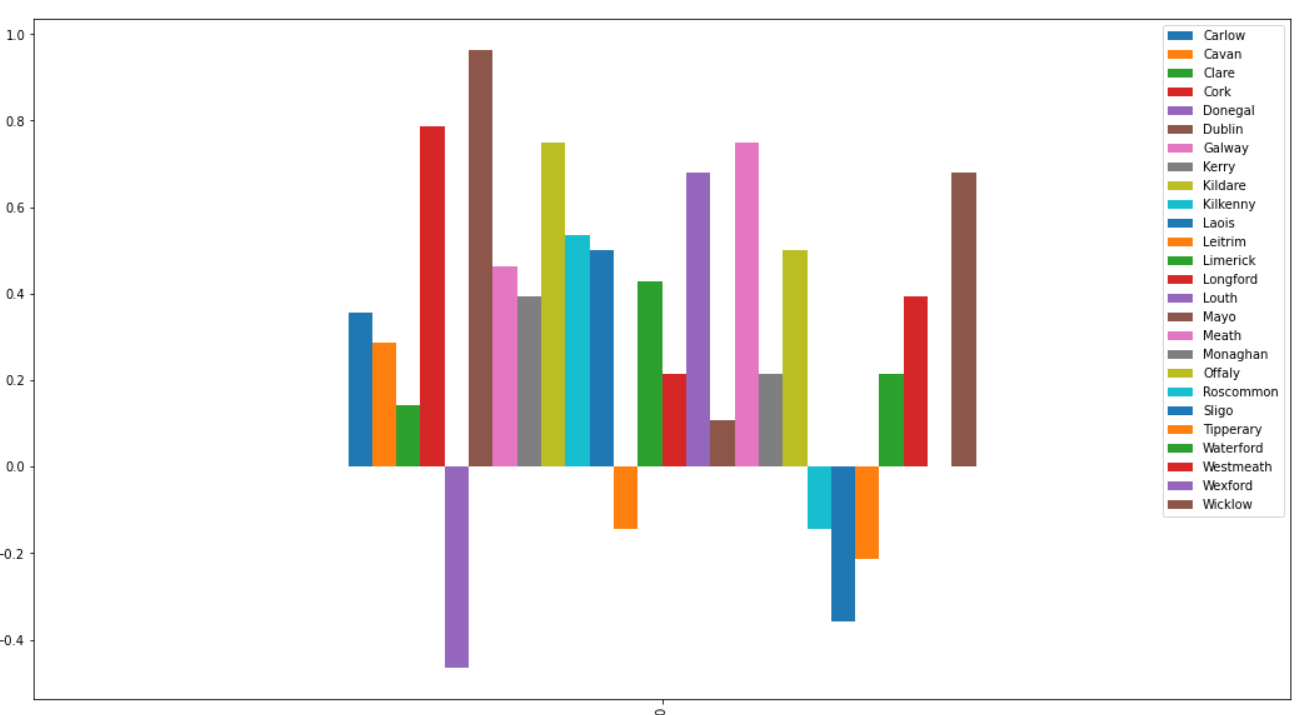
\includegraphics[scale=0.5]{../media/correlations_between_population_and_price_by_county.png}
	\caption{Correlations between population increase and price increase by county}
	\label{fig7}
\end{figure}
\end{document}
